\documentclass[../../main.tex]{subfiles}
\begin{document}

\textit{This section should not list many references}
\textit{Old text (Background)}
\hspace{1pt}

%%%%%%%%
\section{Fluid simulation 101 Background}
%%%%%%%%
{\color{red}\textit{Background. Basic fluid simulation, what do we use it for, what does it mean, method foundation (Lagrangian, Eulerian). What problems do these methods create and how does that affect the use. Other fundamental methods to solve these problems. And once again, problems these methods creates. Computational expensive. }}

In the field of computer graphics, realistic looking scenes and terrain has always been one of the major goals. With the increasing performance and memory capacity of computers, most areas are getting there. However, realistic looking fluid animation is still an area which is too computationally heavy to use efficiently [kanske inte]. A simulation emulates the motion of fluids with the use of either Euler equations or Navier-Stokes equations, or any simpler version or combination of them. Multiple approaches exists with varying positive key aspects and range in complexity from computational expensive high quality animations, towards simpler real-time particle systems.

Eulerian or grid-based methods are a common choice for simulating fluids in the industry(what industry?) due to higher coherence with the ground reality(really?). The grids are usually cheap because there is no neighbor search. All physical quantities of the fluid are defined on a grid, they are then changed over time, but the grid remains fixed. One can look at it as sitting on the bank of a river and the water pass by. 

Lagrangian methods, on the other hand, move fluid mass around explicitly. The quantities are tied to a small part of the fluid which is tracked through the whole simulation. An analogy would be sitting in a boat and drifting down a river. These methods are usually more computationally expensive. However, they offer advantages on creating small scale features like droplets and splashes because of the free surface not bound to a grid. Further they conserve mass implicitly and are simple to implement. One of these methods, and the one we will explore, is Smooth Particles Hydrodynamics (SPH).


%%%%%%%%
\section{SPH}
%%%%%%%%
As the name implies, SPH uses particles to simulate fluids. Each particle uses the distance to it's neighbours to calculate a density value, this value is then used to compute the forward force and velocity. The new position is calculated by forwarding every particles' current position a small distance, using its velocity and a given time step. 

Seeing as the particles depend on neighbors to calculate their positions, the simulation as a whole depend on the number of particles used. If more (and smaller, for the mass to remain the same) particles are used then finer details can be resolved. However, this increase in particle count will also increase the number of calculations. 

%Not sure if related work
%The computationally demanding part has lead many to find techniques to optimise the SPH method. 

Because most fluids are incompressible the particles should not be able to get too close to each other. [something about poisson equation here methinks. Then something about WCSPH and also something about small density fluctuations needs large stiffness which leads to "large pressure jumps for small density variations and therefore requires small time step". Copied from Boundary handling and adaptive time-stepping for PCISPH intro] 

The time step determine how far the fluid will have come for a number of iterations. Therefore, increasing the time step will also increase the real time simulated if the computation time for each iteration is the same. 

In an attempt to increase the time step Solenthaler and Pajarola developed a Predictive-corrective Incompressible SPH (PCISPH). Den fungerar såhär <blablabla>

To further decrease computation time Solenthaler also did the two-scale resolution method.

Goswamis Regional Time Stepping allows higher time steps which decreases computation time as well. 

We propose a combination of the two seeing as they improve on two different aspects of the PCISPH technique

\begin{figure}[h]
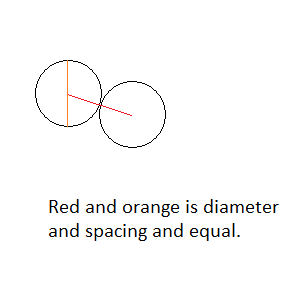
\includegraphics{image/spacing.png}
\caption[Test image]{A image depicting the relationship between particle size and particle spacing.}     
\label{fig:spacing}
\end{figure}

%%%%%%%%
\section{Methods for increasing performance}
%%%%%%%%
{\color{red}\textit{Continuation on the SPH. Mention solutions for earlier mentioned problems. Mention }}




\end{document}